\section{Waves and oscillations}\label{waves-and-oscillations}

\subsection{Sound and Gravity Waves}\label{sound-and-gravity-waves}

We will consider here the simple linearized solution of the atmospheric
primitive equations (\texttt{Eq:SimEq}).

We will suppose a basic state in hydrostatic balance

\[\rho_0 = \frac{p_0}{RT_0}\]

or

\[\frac{1}{p_0}\frac{\partial p_0}{\partial z} = -\frac{g }{RT_0}\]

and

\[H = \frac{RT_0}{g}\]

the scale height of the atmosphere, for typical atmospheric values,
about 8km.

We also suppose an isothermal atmosphere, so that we can solve for the
basic state \(p_0(z) = p_R e^{-z/H}\).

This equations will now be linearized around a basic state with a
constant current \(U=u_0\). The perturbation will have primes
\(u = U + u'\), so substituting and neglecting higher order terms we get
linear equations only for the primes components.

However some terms requires closer consideration. Consider the pressure
gradient terms

\[\frac{1}{(\rho_0 +\rho')}\nabla(p_0+p') +g\hat{k} \approx \frac{1}{(\rho_0 +\rho')}\nabla p' +g\hat{k}=
\frac{1}{\rho_0}\frac{1}{1+\frac{\rho'}{\rho_0}}\nabla p' + g\hat{k} = \frac{1}{\rho_0}\nabla p' + g\hat{k}\]

Where we have used the hydrostatic relation of the basic state to
eliminate the terms containing only the basic state. The potential
temperature can also be linearized:

\[\theta = T \left( \frac{p_R}{p}\right)^\kappa = \frac{p^\kappa_R}{R}\frac{p^{1-\kappa}}{\rho} \approx
\theta_0\left[ 1 + \frac{1}{\gamma}\left(\frac{p'}{p_0}\right) - \frac{\rho'}{\rho_0}\right]\]

since \(\theta = \theta_0 + \theta'\), we have for the equation of state
linearized

\[\frac{\theta'}{\theta_0} = \frac{1}{\gamma}\frac{p'}{p_0} - \frac{\rho'}{\rho_0}\]

where \(\gamma = c_p/c_v\) and remember that \(\kappa = R/c_p\) So the
linearized equation are then

\[\begin{aligned}
&\frac{\partial u}{\partial t} + U\frac{\partial u}{\partial x} + \frac{1}{\rho_0}\frac{\partial p}{\partial x} = 0\\
&\frac{\partial w}{\partial t} + U\frac{\partial w}{\partial x} + \frac{1}{\rho_0}\frac{\partial p}{\partial z}+g\frac{\rho}{\rho_0} = 0\\
&\frac{\partial \rho}{\partial t} + U\frac{\partial \rho}{\partial x}+ w \frac{\partial \rho_0}{\partial z} +\rho_0 (\frac{\partial u}{\partial x} +\frac{\partial w}{\partial z})= 0\\
&\frac{\partial \theta}{\partial t}+ U\frac{\partial \theta}{\partial x} + w \frac{\partial \theta_0}{\partial z}= 0
\end{aligned}\]

considering now

\[\frac{\partial }{\partial z}\frac{p}{p_0} = \frac{1}{p_0}\frac{\partial p}{\partial z} - \frac{p}{p_0^2}\frac{\partial p_0}{\partial z}
= \frac{1}{\rho_0 g H}\frac{\partial p}{\partial z} + \frac{p}{p_0}\frac{1}{H}\]

we get

{\[\frac{\partial u}{\partial t} + U\frac{\partial u}{\partial x} + \frac{1}{\rho_0}\frac{\partial p}{\partial x} = 0\]}

{\[\frac{\partial w}{\partial t} + U\frac{\partial w}{\partial x} +  \frac{1}{\rho_0}\frac{\partial p}{\partial z}  +\rho g= 0\]}

{\[\frac{\partial \rho}{\partial t} + U\frac{\partial \rho}{\partial x} +w \frac{\partial \rho_0}{\partial z}+ \rho_0 (\frac{\partial u}{\partial x} +\frac{\partial w}{\partial z})= 0\]}

{\[\frac{\partial \theta}{\partial t} + U\frac{\partial \theta}{\partial x}+ w \frac{\partial \theta_0}{\partial z}= 0\]}

{\[\frac{\theta}{\theta_0} +\frac{\rho}{\rho_0} + \frac{1}{\gamma}\frac{p}{p_0} = 0\]}

The potential temperature is defined as
\(\theta = T\left(\frac{p_R}{p}\right)^{\kappa}\), where
\(\kappa=R/c_p\). Remembering that
\(N^2 = \frac{1}{\theta_0}\frac{\partial \theta_0}{\partial z} = \frac{\kappa}{H} = \frac{R/c_p}{H}\)
and
\(\frac{\theta}{\theta_0} = \frac{1}{\gamma}\frac{p}{p_0} -\frac{\rho}{\rho_0}\).
For an isothermal basic state at rest (\(U=0\)), then
\(p_0 =\rho_0 R T_0\) where \(T_0\) is constant, so \(p = p_s e^{-z/H}\)
and \(\rho = \rho_s e^{-z/h}\) so we can use eq. \texttt{l5} to
eliminate the potential temperature in eq. \texttt{l4} and use eq.
\texttt{l3} to get

\[\frac{\partial p}{\partial t}  -w\frac{p_0}{H} = -\gamma p_0 \left( \frac{\partial u}{\partial x}+\frac{\partial w}{\partial z} \right)\]

we can use this equation after differentiating eq. \texttt{l1} with
respect to time to get

{\[\left(\frac{\partial^{2} }{\partial t^{2}} -c_s^2\frac{\partial^{2} }{\partial x^{2}}\right)u = c_s^2 \left( \frac{\partial }{\partial z} -\frac{1}{\gamma H} \right)\frac{\partial w}{\partial x}\]}

and then differentiating eq. \texttt{l2} with respect to time and using
eq. \texttt{l3} and eq. \texttt{ll1} we obtain:

{\[\left(\frac{\partial^{2} }{\partial t^{2}} -c_s^2\left[ \frac{\partial^{2} }{\partial z^{2}} -\frac{1}{H}\frac{\partial }{\partial z}\right] \right) w = -c_s^2\left( \frac{\partial }{\partial z} -\frac{\kappa}{H}\right) \frac{\partial u}{\partial x}\]}

The path followed until now is clearly leading towards an equation that
will be fourth order in time. It is to be expected as we are reducing a
system of four equation with single time derivatives. The last step is
the elimination of \(u\) (or also \(w\)) to obtain a single equation.
This can be obtained by noticing the fact that if we operate with

\[-c_s^2\left( \frac{\partial }{\partial z} -\frac{\kappa}{H}\right) \frac{\partial }{\partial x}\]

on eq. \texttt{ll2} and with

\[\left(\frac{\partial^{2} }{\partial t^{2}} -c_s^2\frac{\partial^{2} }{\partial x^{2}}\right)\]

on eq. \texttt{ll2} we can eliminate the term operating on \(u\). Doing
so, we get:

{\[\frac{\partial^4 w}{\partial w^4} -c_s^2\frac{\partial^{2} }{\partial t^{2}} \left(\frac{\partial^{2} }{\partial x^{2}} +\frac{\partial^{2} }{\partial z^{2}}-\frac{1}{H}\frac{\partial }{\partial z}\right)w  -c_s^2 \frac{\kappa g}{H}\frac{\partial^{2} w}{\partial x^{2}} = 0\]}

The term in the single derivative in \(z\) prevents a solution as simple
waves and it is already giving us ahint that there will be more
structure in the vertical. It is to be expected as the basic state has a
vertical structure and so the solution cannot have a pure wavelike form.
Hoever we can separate the wavelike behaviour by a variable
transformation:

\[w = W(x,z,t) e^{z\mu}\]

The substitution will reveal the value for \(\mu\) that is required to
eliminate the first order \(z\) derivative, in this case it is
\(\frac{1}{2H}\). using this value we obtain a simpler equation:

\[\frac{\partial^4 W}{\partial t^4} -c_s^2\frac{\partial^{2} }{\partial t^{2}} \left(\frac{\partial^{2} }{\partial x^{2}} +\frac{\partial^{2} }{\partial z^{2}} -\frac{1}{4H^2}\right)W  -c_s^2 \frac{\kappa g}{H}\frac{\partial^{2} W}{\partial x^{2}} = 0\]

Wave solutions can now be sought by testing

\[W(x,z,t) = Re Ae^{i(kx+mz-\nu t)}\]

that produce the dispersion relation

\[\nu^4 -c_s^2\nu^2\left(k^2+m^2+\frac{1}{4H^2}\right) + c_s^2  N^2 k^2 = 0\]

and the solution

{\[\nu^2 = \frac{1}{2}c_s^2K^2 \left( 1 \pm \sqrt{ 1 - \frac{4N^2k^2}{c_s^2K^4}}\right)\]}

the solution are always real because the term under square root is
always positive. For the isothermal ideal, atmosphere
\(4N^2H^2/c_s^2 \approx 0.8\).

These are not the only solutions. Inspection of \texttt{ll1} and
\texttt{ll2} shows that there is also a solution for \(w=0\) everywhere.
It is a traveling wave in the horizontal ( from eq. \texttt{ll1}) and
the vertical structure is given by eq. \texttt{ll2}, the dispersion
relation is

\[\nu^2 = c_s^2 k^2\]

with a vertical structure

\[u \propto e^{\kappa z/H}\]

so the velocity perturbation grows with height. This is called the
\emph{Lamb wave}.

When the wavenumbers, either \(k\) or \(m\) are very large with respect
to \(H\) we can expand the square root

\[\begin{aligned}
&\nu^2_s = \frac{1}{2}c_s^2K^2 \left( 1 + 1 - \frac{1}{2}\frac{4N^2k^2}{c_s^2K^4}\right)\\
&\nu^2_g = \frac{1}{2}c_s^2K^2 \left( 1 - 1 + \frac{1}{2}\frac{4N^2k^2}{c_s^2K^4}\right)
\end{aligned}\]

or

\[\begin{aligned}
&\nu^2_s = c_s^2K^2 \\
&\nu^2_g =  \frac{N^2k^2}{k^2+m^2+\frac{1}{4H^2}}
\end{aligned}\]

we have added subscripts because the first branch are acoustic waves and
the second gravity waves. We can also see that then the Lamb wave is
also an acoustic wave.

\begin{figure}
 \centering
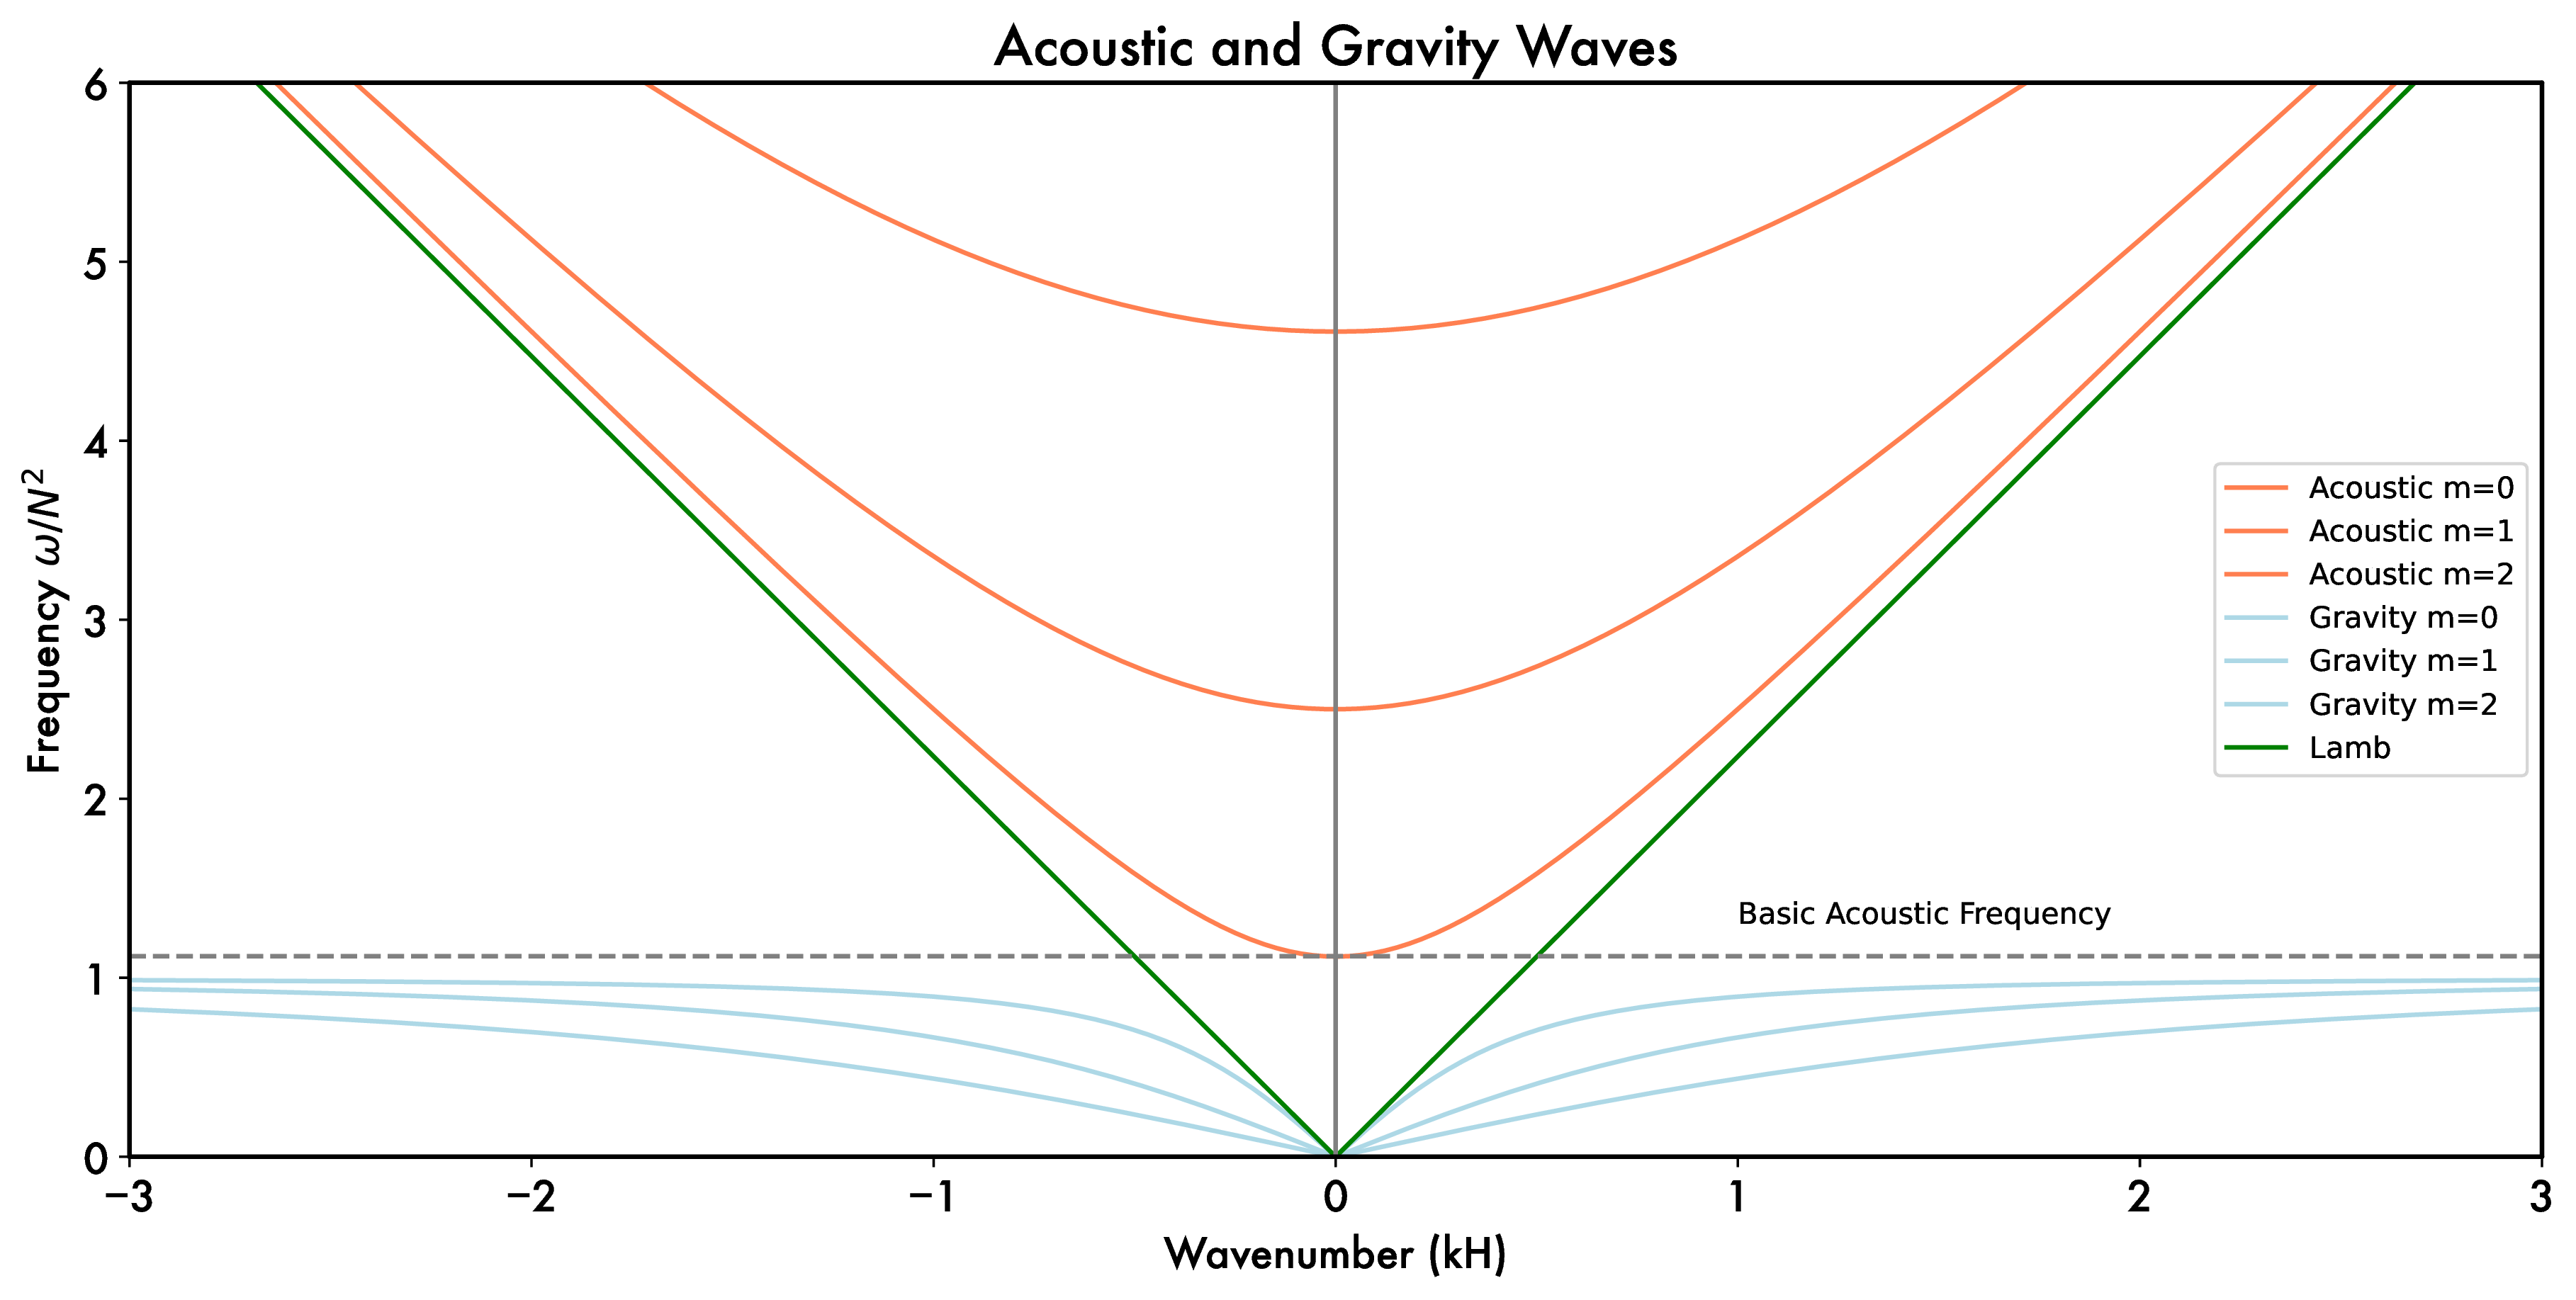
\includegraphics[width = .9 \textwidth, keepaspectratio]{./figs/GD/AcousticWaves.png}
\caption{Dispersion relation for sound and gravity waves.}
\label{fig:disp-rel-sound-gravity-waves}
\end{figure}


Imposing the hydrostatic approximation from the beginning would mean
putting to zero from the start the time time derivative of \(w\) in the
momentum equation in the vertical. This basically equivalent to say that
we are removing the explicit dependence of the vertical velocity on time
and therefore the equation (\texttt{lll}) will be modified as follows.

{\[-c_s^2\frac{\partial^{2} }{\partial t^{2}} \left(\frac{\partial^{2} }{\partial z^{2}}-\frac{1}{H}\frac{\partial }{\partial z}\right)w  -c_s^2 \frac{\kappa g}{H}\frac{\partial^{2} w}{\partial x^{2}} = 0\]}

As a consequence the waves have the same vertical structure, but the
dispersion relation reads:

\[\nu^2 = \frac{N^2k^2}{m^2 + 1 /(4H^2)}\]

this waves are similar to those obtained in the Boussinesq
approximation. The hydrostatic approximation eliminates vertical
propagating sound waves, but the Lamb waves still exists.

\subsection{Barotropic waves}\label{barotropic-waves}

The linearized vorticity equation (\texttt{vorlinsources}) can be solved
in terms of wave solutions

\[\psi = \tilde{\psi}e^{ik(x-ct)}\]

where we have introduced the phase speed \(\omega = c k\),

\[i k (\bar{u}-c)\tilde{\zeta} = -\gamma \tilde{v} = -i k \gamma \tilde{\psi}\]

but the vorticity can be expressed as a streamfunction

\[\tilde{\zeta}=\left( -k^2 +\frac{\partial^{2} }{\partial y^{2}}\right)\tilde{\psi},\]

so

{\[\frac{\partial^{2} \tilde{\psi}}{\partial y^{2}} = \left( k^2 -\frac{\gamma}{\bar{u}-c}\right) \tilde{\psi}\]}

The Eq \texttt{vorlinwave} is an equation of the Sturm-Liouville type
equivalent in form to the Schrödinger equation. Assuming a uniform
basic state \(\bar{u}=U\) and \(\gamma \approx \beta\), we can define a
function with the role of the potential

\[V = \frac{\beta}{U-c} -k^2\]

that depends on the wavenumber of the wave. Solutions to
Eq.(\texttt{vorlinwave}) are exponential also in \(y\),

{\[\tilde{\psi} = \exp{(\pm l y)}\]}

where \(l = \sqrt{- V}\).

\[\begin{aligned}
V= 
\begin{cases}
V > 0 & \text{for}\quad 0 < U-c< \frac{\beta}{k^2}\\
V<0 & \text{for} \quad U-c<0 \quad \text{or}\quad U-c >\frac{\beta}{k^2}
\end{cases}
\end{aligned}\]

Consider the case where the linear equation (\texttt{vorlinwave}) is
forced by a \(\delta\)-function source at some central latitude
\(y =0\), taking the Fourier transform of (\texttt{vorlinwave}) we get

\[(-l^2+V)\hat{\psi} = 1\]

We can obtain the solution by taking the inverse transform, but it will
be very different according to the sign of \(V\) . In the case \(V<0\)
we obtain

\[\begin{aligned}
\tilde{\psi} =
\begin{cases}
\exp\,(ly) & y<0\\
\exp\,(-ly) & y>0\\
\end{cases}
\end{aligned}\]

where we have used \(l=\sqrt(V)\). The solution decays away from the
source for the real exponential case, also called the "trapped wave".
The phase relation between \(\tilde{u}\) and \(\tilde{v}\) are such that
\(\overline{u'v'} = 0\).

Exercise: Prove this relation.

In the case of \(V>0\) the meridional wavenumber \(l\) is complex and
the solution are complex waves

\[\tilde{\psi} = \exp\,( \pm i l y)\]

in this case

\[l^2=\frac{\beta}{U-c} - k^2\]

or

{\[c=U -\frac{\beta}{k^2+l^2}\]}

as expressed in terms of angular frequency

\[\omega = c k = U k -\frac{\beta k}{k^2+l^2},\]

these waves are called Rossby waves.

The group velocity can then be determined from (\texttt{phasespeed})

\[\mathbf{c}_g = (c_x, c_y) = (\frac{\partial \omega}{\partial k},\frac{\partial \omega}{\partial l})\]

for the group velocity we have

\[\begin{aligned}
c_x &= \frac{\partial \omega}{\partial k} =U -\frac{ \beta (l^2-K^2)}{(k^2+l^2)^2}\\
c_y &= \frac{\partial \omega}{\partial l} =\frac{2 \beta k l}{(k^2+l^2)^2}
\end{aligned}\]

The meridional group velocity \(c_y\) is positive for positive
meridional wavenumber \(l\) indicating a poleward propagation and
negative, that is an equatorward propagation, for negative \(l\). The
eddy energy \(\overline{E}\) of the wave is given by

\[\overline{E}=  \frac{1}{2}(\overline{u'^2} +\overline{v'^2})=\frac{1}{4} (k^2+l^2)|\tilde{\psi}|^2\]

so the meridional transport is

\[c_y \overline{E}= \frac{1}{2}\frac{\beta k l }{k^2+l^2}|\tilde{\psi}|^2\]

in a similar way we can estimate readily the momentum transport

\[\overline{u'v'} = \frac{1}{2}\mathrm{Re}\left[ \tilde{u}\tilde{v}^*\right]=\frac{1}{2}\mathrm{Re}\left[ (-il\tilde{\psi})(-ik\tilde{\psi}^*)\right]=-\frac{1}{2}kl|\tilde{\psi}|^2\]


\begin{figure}
\centering
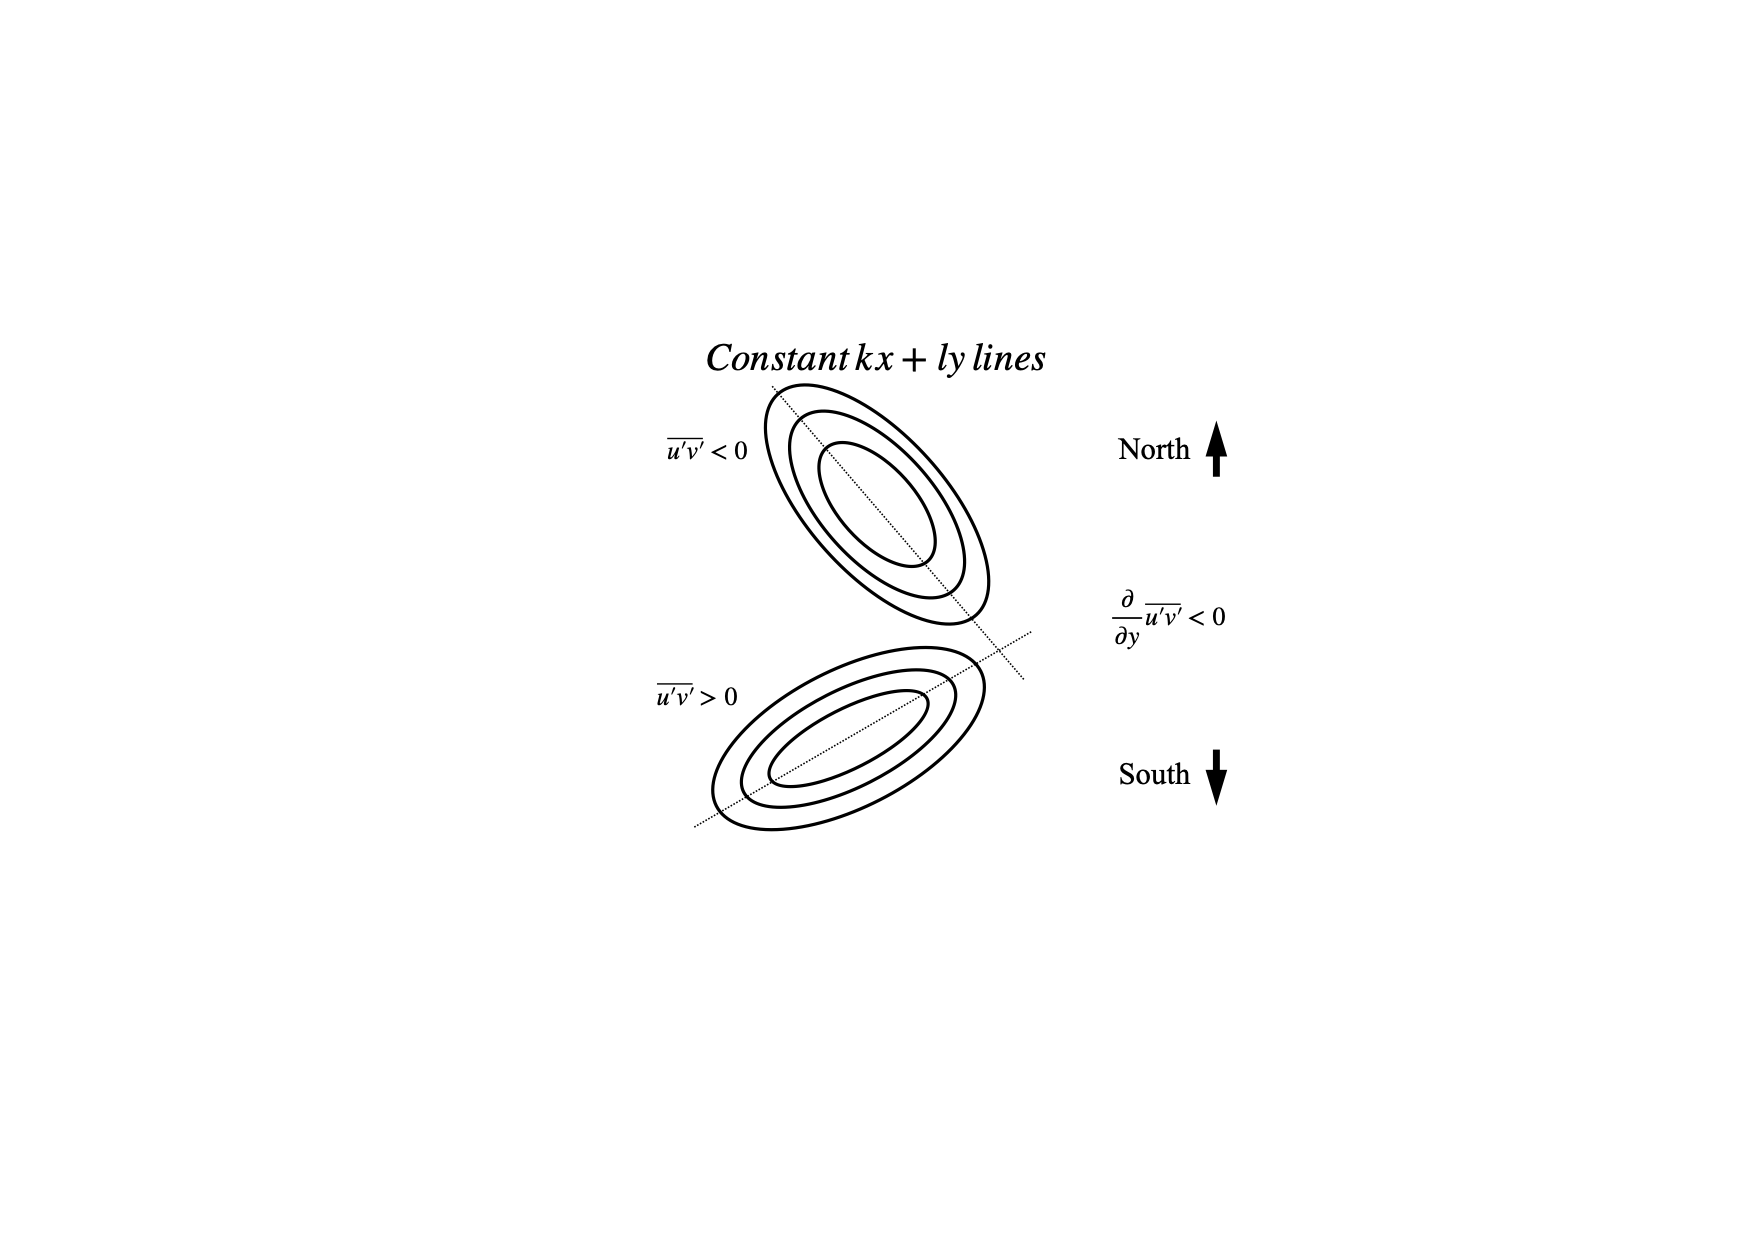
\includegraphics[width =  \textwidth, keepaspectratio]{./figs/GD/BaroSlant.png}
\caption{}
\label{fig:}
\end{figure}

Note that the momentum flux has the opposite direction to the
propagation of the group velocity, a poleward group velocity implies an
equatorward transport of zonal momentum and viceversa. Using
eq.(\texttt{vp}) we can also obtain the result that

{\[\overline{p'v'} = -(\bar{u}-c) (-\frac{1}{2}kl|\tilde{\psi}|^2)= -\frac{\beta}{k^2+l^2}(-\frac{1}{2}kl|\tilde{\psi}|^2) = c_y \overline{E}\]}

This may suggest that we have found a relation for the energy transport,
we have to compute \(\overline{p'u'}\) to check that

\[\overline{p'u'} = -\frac{l}{k}\overline{p'v'}=-\frac{1}{2}\frac{\beta l^2}{k^2+l^2} |\tilde{\psi}|^2\]

is the same as

\[c_x \overline{E}= \frac{\partial \omega}{\partial k}\overline{E}= \frac{1}{4}\beta \frac{k^2-l^2}{k^2+l^2}|\tilde{\psi}|^2.\]

Unfortunately this is not the case and the difference is

\[c_x \overline{E}-\overline{p'u'} = \frac{1}{4}\beta|\tilde{\psi}|^2\]

It is interesting to net that \(\overline{p'u'}\) is always negative,
but the zonal transport \(c_x\overline{E}\) can have both signs.

\subsection{Baroclinic waves}\label{baroclinic-waves}

Consider the baroclinic potential vorticity equation

\[\frac{\partial q}{\partial t} +J(\psi, q) = 0\]

and now linearize around a zonal mean basic state and a constant
stratification (\(N^2 = const\)), then we will have

{\[\frac{\partial q'}{\partial t} = -\bar{u}\frac{\partial q'}{\partial x} - v'\frac{\partial \bar{q}}{\partial y}\]}

where

{\[q'= \nabla^2 \psi'+ f_0 \frac{\partial }{\partial z} \frac{1}{N^2} \frac{\partial \psi'}{\partial z}\]}

and

\[\frac{\partial \bar{q}}{\partial y} = \beta - \frac{\partial^{2} \bar{u}}{\partial y^{2}} -f_0 \frac{\partial }{\partial z} \frac{1}{N^2} \frac{\partial \bar{u}}{\partial z}\]

we are looking for wave solutions

\[\psi = \mathrm{Re}\left[ \tilde{\psi}\,e^{i k(x-ct)}\right]\]

then the steady solution is

\[ik(\bar{u}-c)\left(-k^2\tilde{\psi} +\frac{\partial^{2} \tilde{\psi}}{\partial y^{2}} + f_0 \frac{\partial }{\partial z} \frac{1}{N^2} \frac{\partial \tilde{\psi}}{\partial z}\right) = -ik\tilde{\psi}\frac{\partial \bar{q}}{\partial z}\]

or

\[\frac{\partial^{2} \tilde{\psi}}{\partial y^{2}}  + f_0 \frac{\partial }{\partial z} \frac{1}{N^2} \frac{\partial \tilde{\psi}}{\partial z} = -V(y,z)\tilde{\psi}\]

and

\[V(y,z) = \frac{\displaystyle\frac{\partial \bar{q}}{\partial y}}{\bar{u}-c} - k^2\]

and

\[\frac{\partial \bar{q}}{\partial y} = \beta -\frac{\partial^{2} \bar{u}}{\partial y^{2}} -f_0^2\frac{\partial }{\partial z}\frac{1}{N^2}\frac{\partial \bar{u}}{\partial z}\]

when \(N^2\) is constant we can redefine the vertical coordinate

\[z \to \frac{N }{f_0} z\]

to get

\[\frac{\partial^{2} \tilde{\psi}}{\partial y^{2}} + \frac{\partial^{2} \tilde{\psi}}{\partial z^{2}} = -V \tilde{\psi}\]

with the potential

\[V = \frac{\displaystyle \beta -\frac{\partial^{2} \bar{u}}{\partial y^{2}}-\frac{\partial^{2} \bar{u}}{\partial z^{2}}}{\bar{u}-c} - k^2\]

for constant \(\bar{u}\) and \(N^2\) we can look for wave solutions
\(\tilde{\psi} = \tilde{\psi_0}\exp{i(ly + mz)}\) that provide the
dispersion relation

\[c = \bar{u}-\frac{\beta}{(k^2+l^2+m^2)}\]

We have mow a new group velocity \((c_y, c_z)\) given by

\[c_g = \left(\frac{\partial }{\partial l},\frac{\partial }{\partial m}\right)c k = \frac{\beta k}{(k^2+l^2+m^2)} (l,m)\]

As in the barotropic case \(l>0\) implies poleward propagation and
\(l<0\) equatorward propagation, but now \(m>0\) implies upward
propagation and \(m<0\) implies downward propagation. We can then
estimate the poleward heat flux

{\[\overline{v'\theta'} \approx \mathrm{Re}\left[  i\tilde{\psi}\right]\frac{\partial \tilde{\psi^*}}{\partial z}=\mathrm{Re}\left[ (i)(-im\right]|\tilde{\psi_0}|^2 = m |\tilde{\psi_0}|^2\]}

so upward propagation , \(m > 0\), implies a poleward heat flues,
\(\overline{v'\theta'} > 0\). We can also see that nonpropagating waves,
i.e. trapped waves. or waves that decay exponentially with altitude do
not transport heat because of (\texttt{imflux}).

\begin{figure}
\centering
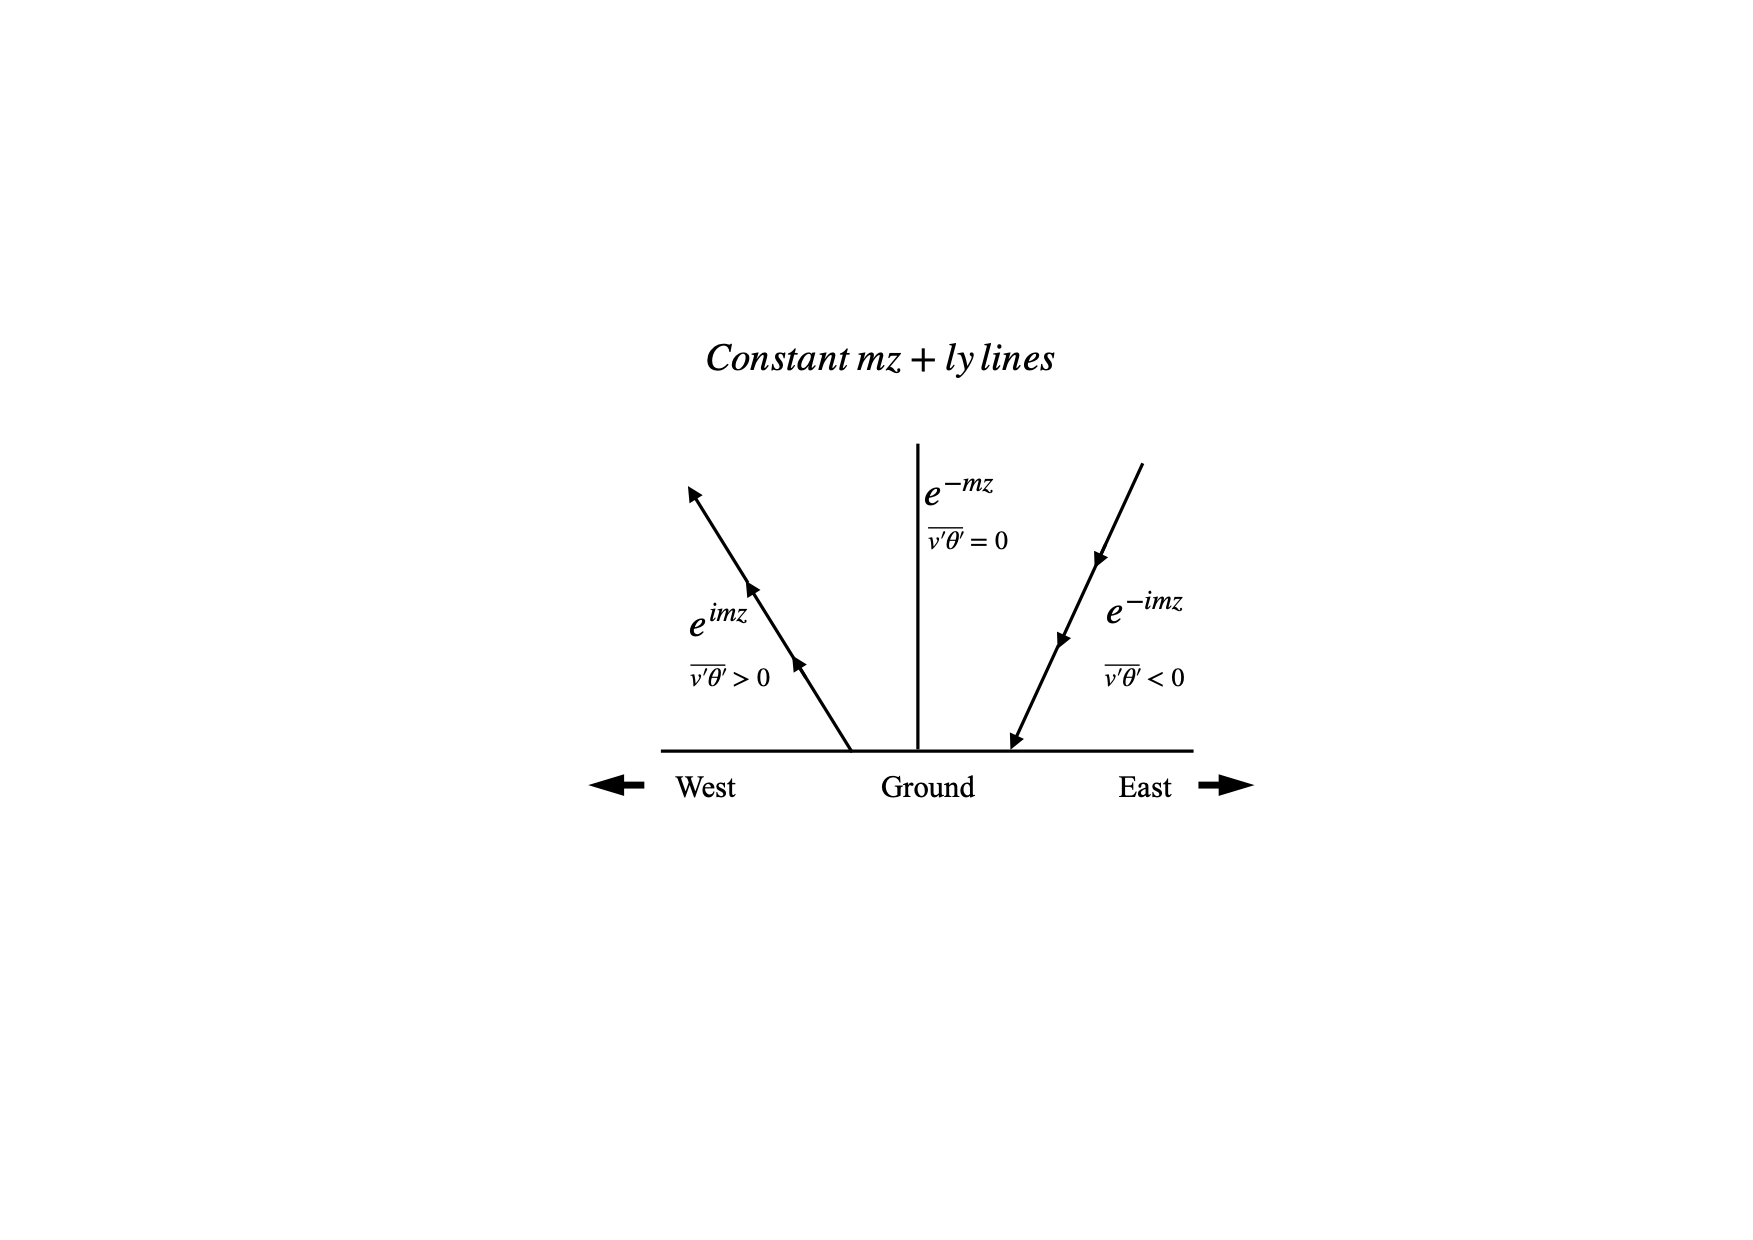
\includegraphics[width= .7 \textwidth]{figs/GD/VertSlant.png}
\caption{}
\label{fig:}
\end{figure}

The condition for vertical propagation then is

\[m^2 = \frac{\beta}{\bar{u}-c} -(k^2+l^2) > 0\]

and we can see that waves can be trapped either by relativeeasterlies
(\(\bar{u}< c\)) or by strong westerlies when
\(\bar{u}> c +\frac{\beta}{k^2+l^2}\). The first vase occurs in summer
stratosphere and the second explians why the winter stratosphere is
dominated by standing waves with very los wavenumbers.

\subsection{Charney-Drazin}\label{charney-drazin}

Considering the linear equation (\texttt{eq:linearq}) with source terms

{\[\frac{\partial q'}{\partial t} = -\bar{u}\frac{\partial q'}{\partial x} - v'\frac{\partial \bar{q}}{\partial y} + X'\]}

but this time we will consider it with the boundary condition on a flat
surface

{\[\frac{\partial \theta'}{\partial t} = -\bar{u}\frac{\partial \theta'}{\partial x} - v'\frac{\partial \bar{\theta}}{\partial y}  + Y'    \qquad  at \,\, z = 0\]}

here we are using the expression (\texttt{eq:qpr}) for the perturbation
potential vorticity and the other quantities are

\[\begin{aligned}
\theta'&= f_0\frac{\partial \psi'}{\partial z}\\
\frac{\partial \bar{q}}{\partial y} &= \beta - \frac{\partial^{2} \bar{u}}{\partial y^{2}} + f_0\frac{\partial }{\partial z}\frac{1}{N^2}\frac{\partial \bar{\theta}}{\partial y}\\
&=\beta - \frac{\partial^{2} \bar{u}}{\partial y^{2}} - f_0^2\frac{\partial }{\partial z}\frac{1}{N^2}\frac{\partial \bar{u}}{\partial z}
\end{aligned}\]

We can write the expression for the fluxes

\[\frac{\partial \overline{q'^2}}{\partial t} = -\overline{v'q'}\frac{\partial \bar{q}}{\partial y} + \overline{v'X'}\]

and

\[\frac{\partial \overline{\theta'^2}}{\partial t} = -\overline{v'\theta'}\frac{\partial \bar{\theta}}{\partial y} + \overline{\theta'Y'}\qquad  at \,\, z = 0\]

these equation show that the potential vorticity flux and the
temperature flux are a function of the wave transient and eventual
explicit sources and sinks. For a steady, conservative flow than

\[\overline{v'q'}=0 \qquad and \qquad \overline{v'\theta'}\qquad  at \,\, z = 0\]

the three dimensional form of the non acceleration theorem, also known
as the Charney-Drazin theorem.

Exercise: Show that similar relation hold for
\(\frac{\partial \bar{u}}{\partial t}\) and
\(\frac{\partial \bar{\theta}}{\partial t}\).
